%Created on: July 8, 2014       Edited by: Wesley Kyle
%Edited on:                     Edited by:
%Edited on:                     Edited by:
%Edited on:                     Edited by:
%Edited on:                     Edited by:
%Edited on:                     Edited by:
%Edited on:                     Edited by:
%Edited on:                     Edited by:


% This is a template for the production of all future lab documents
% 
% IMPORTANT: Edit only between the line "%%%start %%% DO NOT REMOVE THIS LINE"
% and %%%end %%% DO NOT REMOVE THIS LINE
%
% To compile the tex file use the command pdflatex

\documentclass[justified]{tufte-book}
\usepackage{graphicx} % allow embedded images
\setkeys{Gin}{width=\linewidth,totalheight=\textheight,keepaspectratio}
\usepackage{amsmath}  % extended mathematics
\usepackage{booktabs} % book-quality tables
\usepackage{units}    % non-stacked fractions and better unit spacing
\usepackage{multicol} % multiple column layout facilities
\usepackage{fancyvrb} % extended verbatim environments
\fvset{fontsize=\normalsize}% default font size for fancy-verbatim environments
\usepackage{tikz} %for drawing nice pictures
\usepackage{indentfirst}
\usepackage{enumitem}
\usepackage{fancyhdr}
\usepackage{soul}
\usepackage{marvosym}
\pagestyle{fancy}
\usepackage{float}
\allowdisplaybreaks % allows equations to span two pages if needed
\restylefloat{table}
\usetikzlibrary{arrows,snakes,shapes,calc,patterns}
\usetikzlibrary{circuits.ee.IEC}
%\usepackage[T1]{fontenc}
%\usepackage[utf8]{inputenc}

\fancyhf{} % clear all header and footer fields
\fancyfoot[C]{\footnotesize \thepage}
\renewcommand{\headrulewidth}{0pt}
\renewcommand{\footrulewidth}{0pt}


\begin{document}

\chapter{Spectroscopy - Companion Guide}


%%%start %%% DO NOT REMOVE THIS LINE

\section{Equipment}

% first column
\begin{minipage}[t]{0.6\textwidth}
\begin{itemize}[noitemsep]
\item Introductory student spectroscope
\item 600 lines/mm diffraction grating
\item Spectrum tube power supply
\item Hydrogen and Helium Geissler tubes 
\end{itemize}
\end{minipage}
%second column
\begin{minipage}[t]{0.4\textwidth}
\begin{itemize}[noitemsep]
\item Low pressure Sodium lamp
\item Cadmium Osram lamp
\item Laboratory jack
\end{itemize}
\end{minipage}

\section{Setup}
\begin{figure}
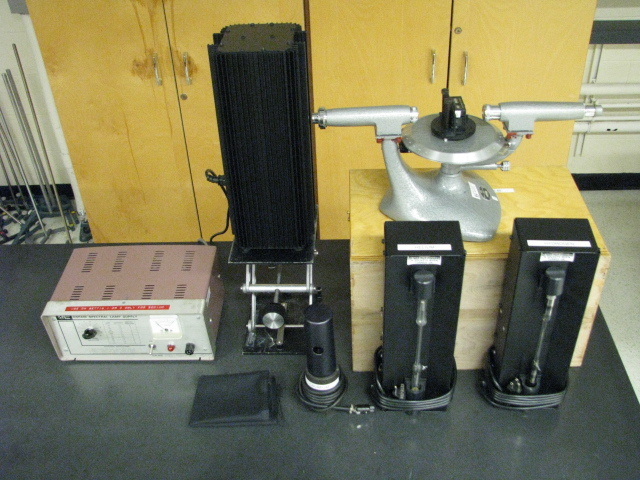
\includegraphics{Spectroscopy-Setup.jpg}
\caption{Equipment Setup}
\label{pic:SPsetup}
\end{figure}

Set up bench as shown in Figure \ref{pic:SPsetup}.

\section{Maintenance}

\begin{enumerate}
\item 
\item 
\end{enumerate}

\section{Critical Points of Failure}

There are currently no known critical points of failure.

\section{Notes to the Instructor}
\begin{enumerate}
\item It is very important for students' success that they calibrate the spectroscope carefully. Of primary importance is ensuring that the grating is perpendicular to the optical axis by checking that the angle of displacement to a reference line on one side is within 0.1$^{\circ}$ of the angle of displacement to the same line on the other side. If the difference is more than this, students will likely achieve unsatisfactory results.
\end{enumerate}

\section{Prelab Questions}
\begin{enumerate}

\item {\bf With Equation 3, compute the numerical value of the Rydberg constant of Hydrogen with units.}\newline

The value of the Rydberg constant for an atom of atomic number, Z, is given by

\small
\begin{align}
R&=\dfrac{m_ee^4Z^2}{8\epsilon_0^2h^3c}\\
&=\dfrac{(9.1\times10^{-31}kg)(1.6\times10^{-19}C)^4(1)^2}{8(8.9\times10^{-12}C^2N^{-1}m^{-2})^2(6.6\times10^{-34}m^2kgs^{-1})^3(3\times10^8ms^{-1})}\\
&=1.0917\times10^{7}m^{-1}
\label{equ:spcg1}
\end{align}
\normalsize

\item {\bf Using Equation 2, compute the visible spectral wavelengths of the Hydrogen spectrum and look up which color these wavelengths correspond to.}\newline

Using the following equation to calculate the wavelength of Balmer series transitions,

\begin{equation}
\dfrac{1}{\lambda}=R\left[\dfrac{1}{2^2}-\dfrac{1}{n^2}\right] \hspace{5mm}n=3,4,5,...
\label{equ:spcg2}
\end{equation}

\begin{table}[ht]
\center
\begin{tabular}{|l|l|l|}
\hline
\multicolumn{1}{|c|}{n} & \multicolumn{1}{c|}{Wavelength (nm)} & \multicolumn{1}{c|}{Colour} \\ \hline
3                       & 656.1                                & red                         \\ \hline
4                       & 486.0                                & indigo                      \\ \hline
5                       & 433.9                                & violet                      \\ \hline
6                       & 410.1                                & violet                      \\ \hline
7                       & 396.9                                & near UV                     \\ \hline
\end{tabular}
\caption{Results for prelab question 2.}
\label{tab:spcg1}
\end{table}

\noindent Students may include the 7-2 transition or not, depending on their definitions for the range of visible light.

\item {\bf If the angle of deviation for a first order spectral line is 20 degrees 17 minutes, what is the wavelength of the corresponding spectral line, assuming the diffraction grating is 600 lines/mm?}\newline

We manipulate the following equation,

\begin{equation}
dsin\theta=m\lambda\hspace{5mm}m=0,\pm1,\pm2,...
\label{equ:spcg3}
\end{equation}

\noindent and set the order, $m=1$, so that

\begin{equation}
\lambda=dsin\theta
\label{equ:spcg4}
\end{equation}

\noindent where $d=1/600$ and $\theta=20.28^{\circ}$. We get the result,

\begin{equation}
\lambda=577.7\hspace{1mm}nm
\label{equ:spcg5}
\end{equation}

\item {\bf Use error analysis to estimate what is the smallest wavelength separation that can be resolved. In otherwords, what uncertainty would be expected for measurements of wavelength with the spectroscope? Assume that the diffraction grating has 600 lines/mm and you are looking at wavelengths around 600nm. Use the error estimates outlined in the error analysis section. Will you be able to reliably resolve all the spectral lines of Helium, Sodium, and Cadmium? If not, list what sources of uncertainty would need to be decreased.}\newline

It is important when answering this question that the ideas of measurement uncertainty and resolution not be conflated, even though the phrasing of the questions appears to do so. The idea here is that a doublet may be able to be resolved in the student introductory spectrometer but the uncertainty in the measurement might preclude the ability to accurately measure the difference in angle between them. We then need to propagate the uncertainties listed in the Error Analysis section to find the uncertainty in any wavelength measurement. If two lines fall within this uncertainty, we can say that we would be unable to distinguish them {\it by measurement}. 

We begin by determining the linewidth, d, and the deviation angle, $\theta$, along with their corresponding uncertainties, u(d) and u($\theta$), respectively.

\begin{equation}
d=\dfrac{1}{600000\hspace{1mm}lines/m}=1.67\times10^{-6}
\label{equ:spcg6}
\end{equation}



\begin{align}
u(d)&=\dfrac{\partial d}{\partial n_{lines}}\cdot u(n_{lines})\\
&=\dfrac{1}{(600000\hspace{1mm}lines/m)^2}\cdot 5000\hspace{1mm}lines/m\\
&=1.39\times10^{-8}
\label{equ:spcg7}
\end{align}

\noindent So the line spacing, d, is expressed as $1.67\times10^{-6}\pm1.39\times10^{-8}$ m. Moving on to the angle, $\theta$, we are told that we are observing around wavelengths of 600 nm.

\begin{align}
\theta&=sin^{-1}(\dfrac{\lambda}{d})=sin^{-1}\left(\dfrac{600\times10^{-9}}{1.67\times10^{-6}}\right)\\
&=0.367\pm 0.0035\hspace{1mm}rad
\label{equ:spcg8}
\end{align}

\noindent We are told that the uncertainty in any angle measurement is $\pm 0.1^{\circ}$ which is $\pm 0.0035$ radians.

The expression we use for finding the uncertainty in the wavelength is derived from Equation \ref{equ:spcg3} with the order, m, taken to be $1$. We then apply the partial derivative formula for uncertainty and add the terms in quadrature.

\begin{align}
u(\lambda)&=\sqrt{\left(\dfrac{\partial \lambda}{\partial d}\cdot u(d)\right)^2+\left(\dfrac{\partial \lambda}{\partial \theta}\cdot u(\theta)\right)^2}\\
&=\sqrt{(sin(\theta)\cdot u(d))^2+(dcos(\theta)\cdot u(\theta))^2}\\
&=7.39\hspace{1mm}nm
\label{equ:spcg9}
\end{align}

So our uncertainty in any measurement of angle expresses itself as an uncertainty of $\pm5.65$ nm in the wavelength. This means that for the red, yellow, and lime Sodium doublets, the uncertainty of each measurement is larger than the separation between the lines.

\end{enumerate}


\section{Data Requirements}
\begin{enumerate}

\item {\bf Notes and observations from the setup and alignment of the spectroscope (steps 1-7).}\newline

Collimator and telescope were focused, crosshairs were brought into focus, grating table was balanced, and the grating was aligned to be perpendicular to the optical axis.

\item {\bf A table of data for the Hydrogen lamp as a performance check of the diffraction grating, including calibration source, center angle, colour, angle of diffraction, angle of deviation, and theoretical wavelength together with errors (procedure step 9).}\newline

\begin{table}[ht]
\center
\begin{tabular}{|l|l|l|l|l|l|}
\hline
\multicolumn{1}{|c|}{Calibration Source} & \multicolumn{1}{c|}{$\theta_0$ (deg)} & \multicolumn{1}{c|}{Colour} & \multicolumn{1}{c|}{$\theta$ (deg)} & \multicolumn{1}{c|}{$\Delta\theta$ (deg)} & \multicolumn{1}{c|}{$\lambda$ (nm)} \\ \hline
Hydrogen                                 & 207.8                                 & violet                      & 222.2                               & 14.4$\pm$0.2                              & 414.5$\pm$6.61                      \\ \hline
                                         &                                       & violet                      & 223.0                               & 15.2$\pm$0.2                              & 437.0$\pm$6.69                      \\ \hline
                                         &                                       & indigo                      & 224.9                               & 17.1$\pm$0.2                              & 490.1$\pm$6.90                      \\ \hline
                                         &                                       & red                         & 231.2                               & 23.4$\pm$0.2                              & 661.9$\pm$7.68                      \\ \hline
\end{tabular}
\caption{Data collected for Hydrogen calibration.}
\label{tab:spcg2}
\end{table}

\item {\bf A rough graph of $\lambda$ (theoretical wavelength) versus sin($\theta$) and a value with error for the line spacing, d, of the diffraction grating (procedure step 9).}\newline

\begin{figure}
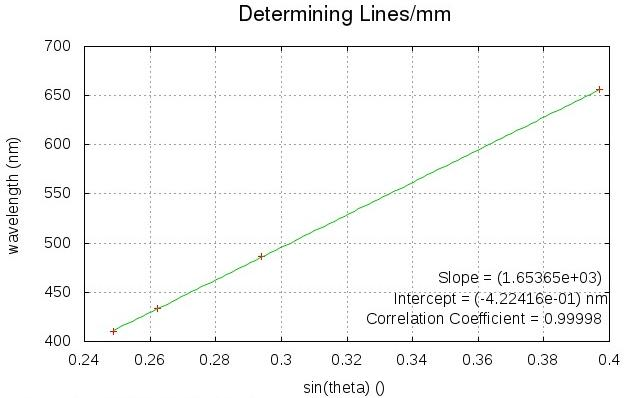
\includegraphics{Spectroscopy-calibration.jpg}
\caption{Rough linear plot of $\lambda$ vs. sin($\theta$). Here the slope is 1.65 $\mu$m which corresponds to 604.7 lines/mm, within the uncertainty of the manufacturers value of 600$\pm$5 lines/mm.}
\label{fig:spcg1}
\end{figure}

\item {\bf Tables of data from the Helium, Sodium, and Cadmium lamps, including center angle, colour, angle of diffraction, angle of deviation (procedure steps 10 and 11).}\newline

\begin{table}[ht]
\center
\begin{tabular}{|l|l|l|l|l|l|}
\hline
\multicolumn{1}{|c|}{Source} & \multicolumn{1}{c|}{$\theta_0$ (deg)} & \multicolumn{1}{c|}{Colour} & \multicolumn{1}{c|}{$\theta$ (deg)} & \multicolumn{1}{c|}{$\Delta\theta$ (deg)} & \multicolumn{1}{c|}{$\lambda$ (nm)} \\ \hline
Helium                                   & 207.8                                 & violet                      & 223.5                               & 15.7$\pm$0.2                              & 451.0$\pm$6.75                      \\ \hline
                                         &                                       & blue                        & 224.4                               & 16.6$\pm$0.2                              & 476.1$\pm$6.84                      \\ \hline
                                         &                                       & green                       & 225.5                               & 17.7$\pm$0.2                              & 506.7$\pm$6.97                      \\ \hline
                                         &                                       & yellow                      & 228.7                               & 20.9$\pm$0.2                              & 594.6$\pm$7.36                      \\ \hline
                                         &                                       & red                         & 231.7                               & 23.9$\pm$0.2                              & 675.2$\pm$7.75                      \\ \hline
\end{tabular}
\caption{Data collected for Helium.}
\label{tab:spcg3}
\end{table}


\begin{table}[ht]
\center
\begin{tabular}{|l|l|l|l|l|l|}
\hline
\multicolumn{1}{|c|}{Source} & \multicolumn{1}{c|}{$\theta_0$ (deg)} & \multicolumn{1}{c|}{Colour} & \multicolumn{1}{c|}{$\theta$ (deg)} & \multicolumn{1}{c|}{$\Delta\theta$ (deg)} & \multicolumn{1}{c|}{$\lambda$ (nm)} \\ \hline
Cadmium                                  & 207.8                                 & blue                        & 224.2                               & 16.4$\pm$0.2                              & 470.6$\pm$6.82                      \\ \hline
                                         &                                       & light blue                  & 224.6                               & 16.8$\pm$0.2                              & 481.7$\pm$6.87                      \\ \hline
                                         &                                       & green                       & 225.7                               & 17.9$\pm$0.2                              & 512.3$\pm$6.99                      \\ \hline
                                         &                                       & red                         & 230.7                               & 22.9$\pm$0.2                              & 648.5$\pm$7.61                      \\ \hline
\end{tabular}
\caption{Data collected for Cadmium.}
\label{tab:spcg4}
\end{table}


\begin{table}[ht]
\center
\begin{tabular}{|l|l|l|l|l|l|}
\hline
\multicolumn{1}{|c|}{Source} & \multicolumn{1}{c|}{$\theta_0$ (deg)} & \multicolumn{1}{c|}{Colour} & \multicolumn{1}{c|}{$\theta$ (deg)} & \multicolumn{1}{c|}{$\Delta\theta$ (deg)} & \multicolumn{1}{c|}{$\lambda$ (nm)} \\ \hline
Sodium                                   & 207.8                                 & lime                        & 227.9                               & 20.1$\pm$0.2                              & 572.8$\pm$7.26                      \\ \hline
                                         &                                       & yellow                      & 228.7                               & 20.9$\pm$0.2                              & 594.6$\pm$7.36                      \\ \hline
                                         &                                       & red                         & 229.7                               & 21.9$\pm$0.2                              & 621.6$\pm$7.48                      \\ \hline
\end{tabular}
\caption{Data collected for Sodium.}
\label{tab:spcg5}
\end{table}

\section{Calculations and Analysis}

\item {\bf A graph of $\lambda$ (theoretical wavelength) versus sin($\theta$) and a value, with error, for the line spacing, d, of the diffraction grating.}\newline

See Q7.

\item {\bf Tables of data from the Helium, Sodium, and Cadmium lamps, including center angle, colour, angle of diffraction, angle of deviation, and measured wavelength, together with errors.}\newline

See Q8.

\section{Discussion}

\item {\bf A comparison of the measured diffraction grating spacing with the expected value.}\newline

Results of analysis showed that the expected grating spacing did not match the experimentally determined value to within uncertainty. A larger value for uncertainty or an adjusted expected value may be necessary.

\item {\bf A discussion of the performance of the diffraction grating and which method of wavelength determination is preferred; using the manufacturers specified grating spacing or the measured grating spacing instead? Which error is preferred; the one in the error analysis section or the measured value?}\newline

Experimentally determined values for line spacing and uncertainty are preferable to manufacturers stated values for both pragmatic and ideological reasons. Pragmatically, one desires to be sure of the physical parameters of one's equipment as they really are, not as they ought to be. Ideologically, one wishes to be able to point to experimentally verifiable data to support methods and conclusions.

\item {\bf A comparison of the spectral wavelengths measured for Helium, Sodium, and Cadmium, with the accepted values.}\newline

Literature values of spectral lines for Sodium, Cadmium, and Helium were obtained from Table 1 in the laboratory manual.


\begin{table}[ht]
\center
\begin{tabular}{|l|l|l|l|}
\hline
\multicolumn{1}{|c|}{Source} & \multicolumn{1}{c|}{Theoretical $\lambda$ (nm)} & \multicolumn{1}{c|}{Experimental $\lambda$ (nm)} & \multicolumn{1}{c|}{Error (nm)} \\ \hline
Helium                       & 447.1479                                        & 451.0006                                   & 3.8526                          \\ \hline
                             & 471.3146                                        & 476.1470                                         & 4.8324                          \\ \hline
                             & 501.5678                                        & 506.7215                                         & 5.1537                          \\ \hline
                             & 587.562                                         & 594.5630                                         & 7.0010                          \\ \hline
                             & 667.815                                         & 675.2357                                         & 7.4207                          \\ \hline
\end{tabular}
\caption{A comparison of expected and experimental values for the wavelength of spectral lines of Helium.}
\label{tab:spcg6}
\end{table}


\begin{table}[ht]
\center
\begin{tabular}{|l|l|l|l|}
\hline
\multicolumn{1}{|c|}{Source} & \multicolumn{1}{c|}{Theoretical $\lambda$ (nm)} & \multicolumn{1}{c|}{Experimental $\lambda$ (nm)} & \multicolumn{1}{c|}{Error (nm)} \\ \hline
Cadmium                       & 467.8149                                        & 470.5689                                         & 2.7540                          \\ \hline
                             & 479.9912                                        & 481.7194                                         & 1.7282                          \\ \hline
                             & 508.5822                                        & 512.2608                                         & 3.6786                          \\ \hline
                             & 643.8470                                        & 648.5396                                         & 4.6926                          \\ \hline
\end{tabular}
\caption{A comparison of expected and experimental values for the wavelength of spectral lines of Cadmium.}
\label{tab:spcg7}
\end{table}

Because Sodium contains 3 sets of doublets which are visibly distinguished but unresolved in the sense that they cannot be accurately measured as separate lines, we have taken the average value of each doublet to represent a hypothetical single line which is what the observer measures. The difference between these values and the experimentally measured values is taken as the measurement error.

\begin{table}[ht]
\center
\begin{tabular}{|l|l|l|l|l|}
\hline
\multicolumn{1}{|c|}{Source} & \multicolumn{1}{c|}{$\lambda_{lit}$ (nm)} & \multicolumn{1}{c|}{$\lambda_{avg}$ of Doublet} & \multicolumn{1}{c|}{$\lambda_{exp}$ (nm)} & \multicolumn{1}{c|}{Error (nm)} \\ \hline
Sodium                       & 568.2633                                        & 568.5419                                          & 572.7659                                         & 4.2240                    \\ \hline
                             & 568.8205                                        &                                                   &                                                  &                                 \\ \hline
                             & 588.995                                         & 589.2937                                          & 594.5630                                         & 5.2693                     \\ \hline
                             & 589.5924                                        &                                                   &                                                  &                                 \\ \hline
                             & 615.4225                                        & 615.7486                                          & 621.6460                                         & 5.8974                    \\ \hline
                             & 616.0747                                        &                                                   &                                                  &                                 \\ \hline
\end{tabular}
\caption{A comparison of expected and experimental values for the wavelength of spectral lines of Sodium.}
\label{tab:spcg8}
\end{table}




\end{enumerate}




%%%end %%% DO NOT REMOVE THIS LINE

\end{document}